\documentclass[border=6pt]{standalone}
\usepackage{pgfplots}
\pgfplotsset{compat=1.17}
\usepackage{mathptmx}
\definecolor{navy}{RGB}{20,52,110}
\definecolor{accent}{RGB}{14,110,120}
\definecolor{gray70}{RGB}{130,130,130}
\begin{document}
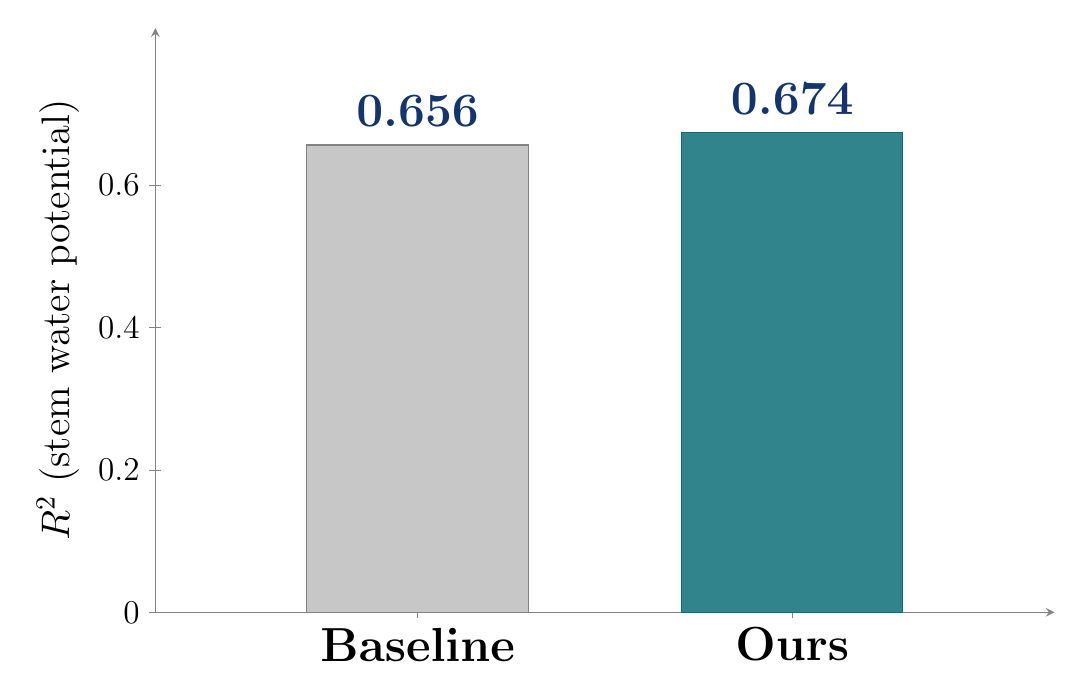
\begin{tikzpicture}
\begin{axis}[
    width=13cm, height=9cm,
    ymin=0, ymax=0.82,
    xmin=0.3, xmax=2.7,
    ytick={0,0.2,0.4,0.6},
    ylabel={\Large $R^2$ (stem water potential)},
    xtick={1,2},
    xticklabels={Baseline,Ours},
    xticklabel style={font=\LARGE\bfseries},
    yticklabel style={font=\large},
    ylabel style={font=\large},
    axis lines=left,
    clip=false,
    axis line style={gray70},
    tick style={gray70},
]
\addplot[ybar, bar width=80pt, draw=gray70, fill=gray70!45] coordinates {(1,0.656)};
\addplot[ybar, bar width=80pt, draw=accent, fill=accent!85] coordinates {(2,0.674)};
\node[font=\LARGE\bfseries, color=navy] at (axis cs:1,0.656) [anchor=south, yshift=3pt] {0.656};
\node[font=\LARGE\bfseries, color=navy] at (axis cs:2,0.674) [anchor=south, yshift=3pt] {0.674};
\end{axis}
\end{tikzpicture}
\end{document}
